\documentclass{beamer}
\usetheme{Boadilla}
\setbeamertemplate{navigation symbols}{}

\usepackage[light]{antpolt}
\usepackage{hyperref}
\usepackage{tikz}

\DeclareMathOperator{\M}{\mathcal M}
\DeclareMathOperator{\N}{\mathcal N}
\DeclareMathOperator{\G}{\mathcal G}

\newcommand{\eq}[1]{\begin{align*} #1 \end{align*}}
\newcommand{\game}[8]{\eq{\begin{array}{ccccccccc} \text{I} & #1 && #3 && #5 && #7\\ \text{II} && #2 && #4 && #6 && #8 \end{array}}}

\title[Virtual large cardinals]{Virtual large cardinals\\ {\small\textsc{European Set Theory Conference, Vienna}}}
\author[Dan Saattrup Nielsen]{Dan Saattrup Nielsen\\ University of Bristol}
\date{July 2019}

\begin{document}

{
\setbeamertemplate{background canvas}{
  \tikz[remember picture, overlay]
  \node[opacity=0.5] at (7.2, -7.5){
    \includegraphics[width = 3.5cm]{gfx/alumni.png}
    \hspace{3.0cm}
    \includegraphics[width = 6cm]{gfx/epsrc.jpg}
  };
}

\begin{frame}
	\titlepage
\end{frame}
}

\begin{frame}{What are they?}
  \begin{block}{Rough definition}
    A large cardinal $\kappa$ defined via \textit{set-sized} elementary embeddings is \textbf{virtual} if the elementary embeddings exist in a generic extension.
  \end{block}

  \begin{center}
    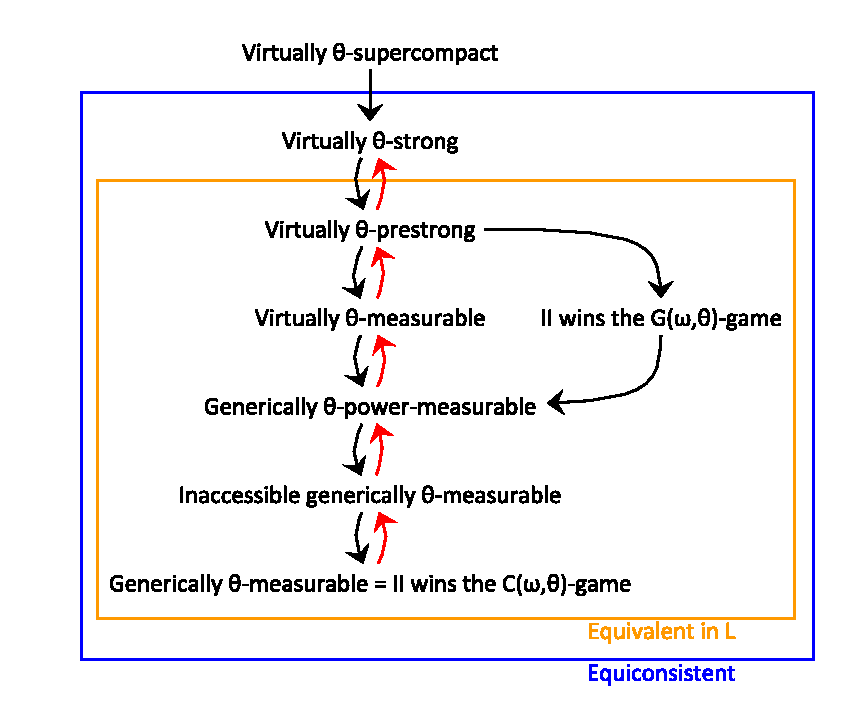
\includegraphics[scale=0.17]{gfx/virtual.jpg}
  \end{center}
\end{frame}

\begin{frame}{What are they?}
  \begin{block}{Rough definition}
    A large cardinal $\kappa$ defined via \textit{set-sized} elementary embeddings is \textbf{generic} if the elementary embeddings {\color{red} and the target model} exist in a generic extension.
  \end{block}

  \begin{center}
    \includegraphics[scale=0.17]{gfx/generic.jpg}
  \end{center}
\end{frame}

\begin{frame}{Why should we care?}
  \begin{block}{Theorem (Schindler '00)}
    A virtually strong cardinal is equiconsistent with $\text{Th}(L(\mathbb R))$ being unchangeable by proper forcing.
  \end{block}
  
  \pause

  \begin{block}{Theorem (Schindler-Wilson '18)}
    A virtually Shelah cardinal is equiconsistent with every universally Baire set of reals having the perfect set property.
  \end{block}

  \pause
  
  \begin{block}{Theorem (Wilson '19)}
    A virtually Vop\v enka cardinal is equiconsistent with $\Theta=\omega_2$ and ${\bf\Sigma}^1_2$ being the class of all $\omega_1$-Suslin sets.
  \end{block}
\end{frame}

\begin{frame}{Where are they?}
  \begin{center}
    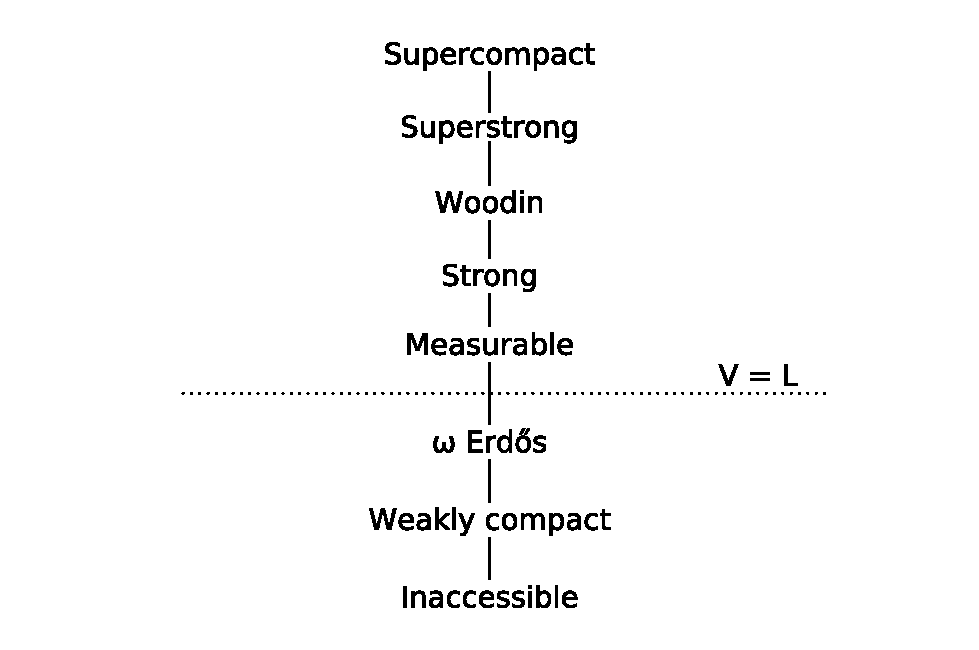
\includegraphics[scale=.16]{gfx/hierarchy.jpg}
  \end{center}
\end{frame}

\begin{frame}{How do they behave?}
  \begin{block}{Theorem (Gitman)}
    Virtually strongs are equivalent to virtually supercompacts.
  \end{block}

  \pause

  \begin{block}{Theorem (N.)}
    Virtually measurables are equiconsistent with virtually strongs.
  \end{block}

  \pause

  \begin{block}{Theorem (Schindler-N.)}
    There exists a game representation for the generically measurables.
  \end{block}
\end{frame}

\begin{frame}{How do they behave level by level?}
  \begin{center}
    \includegraphics[scale=.18]{gfx/lbl_virtual.jpg}
  \end{center}
\end{frame}

\begin{frame}{Future work}
  \begin{enumerate}
    \item Are virtually $\theta$-strongs equivalent to virtually $\theta$-supercompacts?
    \pause\item How do virtually Woodin cardinals behave? \pause Vop\v enka cardinals?
    \pause\item Virtualising small embedding cardinals like Ramsey cardinals and below?
    \pause\item Game characterisations of other generic large cardinals?
    \pause\item Indestructibility properties?
  \end{enumerate}
\end{frame}

\end{document}
